\section{Order\-Xover Class Reference}
\label{class_order_xover}\index{OrderXover@{OrderXover}}
Order Crossover.  


{\tt \#include $<$order\_\-xover.h$>$}

Inheritance diagram for Order\-Xover::\begin{figure}[H]
\begin{center}
\leavevmode
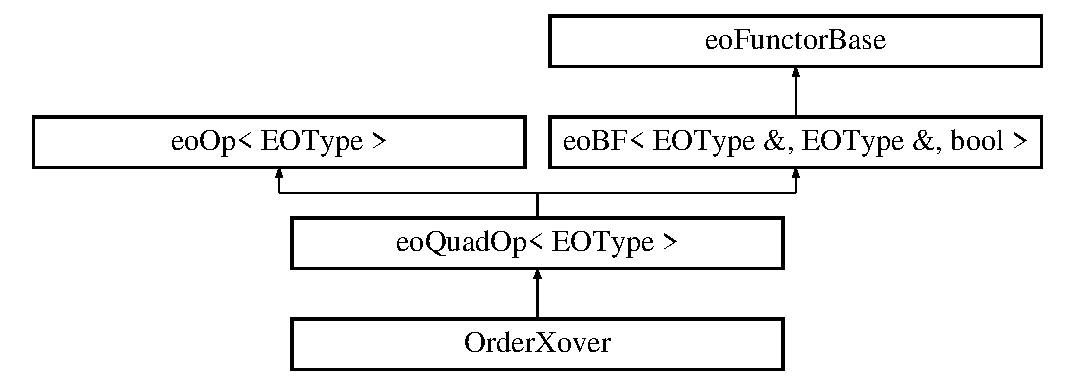
\includegraphics[height=4cm]{class_order_xover}
\end{center}
\end{figure}
\subsection*{Public Member Functions}
\begin{CompactItemize}
\item 
bool \bf{operator()} (\bf{Route} \&\_\-\_\-route1, \bf{Route} \&\_\-\_\-route2)\label{class_order_xover_0ff6aada669eb8173322ed68cda1ac61}

\end{CompactItemize}
\subsection*{Private Member Functions}
\begin{CompactItemize}
\item 
void \bf{cross} (const \bf{Route} \&\_\-\_\-par1, const \bf{Route} \&\_\-\_\-par2, \bf{Route} \&\_\-\_\-child)\label{class_order_xover_d2bf90b5f46ac4a344777e17bc5f364d}

\end{CompactItemize}


\subsection{Detailed Description}
Order Crossover. 



Definition at line 45 of file order\_\-xover.h.

The documentation for this class was generated from the following files:\begin{CompactItemize}
\item 
order\_\-xover.h\item 
order\_\-xover.cpp\end{CompactItemize}
